\documentclass[12pt,a4paper,twoside]{book}
\usepackage{graphicx}
\usepackage{setspace}	%double spacing for text, single for captions, footnotes, etc.
%\usepackage{hypernat} 	%substitut de cite que permet fer hyperlinks
\usepackage{natbib}		% substituye a 'hypernat' que funciona en Windows.
\usepackage[english]{babel}
\usepackage[utf8]{inputenc}
\usepackage{color}
\usepackage{hhline} 		% extended styles for tables
\usepackage{multirow}
\usepackage{subfigure}
\usepackage{acronym}
\usepackage{hyperref}
\usepackage{amsmath,amsmath,amssymb} 
\usepackage{fancyhdr}
\usepackage{epsfig, amsmath}
\usepackage{algorithm}
\usepackage{algorithmic}
\usepackage{refcount}


\graphicspath{ {./images/} }


% general settings
\hypersetup{
	linktocpage=true,
	colorlinks=true,
	linkcolor=blue,
	citecolor=blue,
}
\definecolor{Hgray}{gray}{0.6}

\newenvironment{definition}[1][Definition]{\begin{trivlist}
\item[\hskip \labelsep {\bfseries #1}]}{\end{trivlist}}

\setlength{\topmargin}{0cm}
\setlength{\textheight}{23cm}
\setlength{\textwidth}{17cm}
\setlength{\oddsidemargin}{0cm}
\setlength{\evensidemargin}{0cm}
\setlength{\headheight}{1cm}

% indica que las 'sub-sub-sections' sean numeradas y aparezcan en el indice
\setcounter{secnumdepth}{3}
\setcounter{tocdepth}{2}

% settings for code
\renewcommand{\algorithmicrequire}{\textbf{Entrada: }}
\renewcommand{\algorithmicensure}{\textbf{Salida: }}

%%%%%%%%%%%%
% DOCUMENT %
%%%%%%%%%%%%
\begin{document}

% portada
\newpage
\thispagestyle{empty}

\baselineskip 2em

%\vspace*{1cm}

\centerline{
\includegraphics[width=0.6\textwidth]{images/UOC-logo}}
\begin{center}
\textsc{Universitat Oberta de Catalunya (UOC) \\
 Máster Universitario en Ciencia de Datos (\textit{Data Science})\\}

%\centerline {\pic{UOC}{4cm}}

\vspace*{1.5cm}

\textsc{\Large TRABAJO FINAL DE MÁSTER}

\vspace*{0.5cm}

\textsc{\large Área: 4}


%\textbf{\Huge VirtualTechLab Model: }

\vspace*{2.0cm}

\textbf{\Large Answer generation for retrieval based questions for breastfeeding advice from noisy, 
user-generated content.}

% \textbf{\large xxx subtítulo (en caso de existir) xxx}

\vspace{2.5cm}
\baselineskip 1em

\baselineskip 2em
-----------------------------------------------------------------------------\\
Author:     Arcadi Gonzalez Graells\\
Tutor:      Elisenda Bonet Carne\\
Professor:   Nadjet Bouayad-Agha \\
-----------------------------------------------------------------------------\\
\vspace*{1.5cm}
London, \today

\end{center}

\newpage
\pagestyle{empty}
\hfill

\newpage
% abstract
\pagenumbering{roman} 
\setcounter{page}{1} 
\pagestyle{plain}

%%%%%%%%%%%%%%%%
%%% CREDITOS %%%
%%%%%%%%%%%%%%%%
%\chapter*{Créditos/Copyright}

%Una página con la especificación de créditos/copyright para el proyecto (ya sea aplicación por un lado y documentación por el otro, o unificadamente), así como la del uso de marcas, productos o servicios de terceros (incluidos códigos fuente). Si una persona diferente al autor colaboró en el proyecto, tiene que quedar explicitada su identidad y qué hizo.

%A continuación se ejemplifica el caso más habitual, aunque se puede modificar por cualquier otra alternativa:

%\vspace{1cm}

% \begin{figure}[ht]
%     \centering
% 	
\includegraphics[scale=1]{images/license.png}
% \end{figure}

% Esta obra está sujeta a una licencia de Reconocimiento -  NoComercial - SinObraDerivada

% \href{https://creativecommons.org/licenses/by-nc-nd/3.0/es/}{3.0 España de CreativeCommons}.

%%%%%%%%%%%%%
%%% FICHA %%%
%%%%%%%%%%%%%
% \chapter*{FICHA DEL TRABAJO FINAL}

% \begin{table}[ht]
% 	\centering{}
% 	\renewcommand{\arraystretch}{2}
% 	\begin{tabular}{r | l}
% 		\hline
% 		Título del trabajo: & Descriptivo del trabajo\\
% 		\hline
%         Nombre del autor: & Nombre y dos apellidos\\
% 		\hline
%         Nombre del colaborador/a docente: & Nombre y dos apellidos\\
% 		\hline
%         Nombre del PRA: & Nombre y dos apellidos\\
% 		\hline
%         Fecha de entrega (mm/aaaa): & MM/AAAA\\
% 		\hline
%         Titulación o programa: & Plan de estudios\\
% 		\hline
%         Área del Trabajo Final: & El nombre de la asignatura de TF\\
% 		\hline
%         Idioma del trabajo: & Catalán, español o inglés\\
% 		\hline
%         Palabras clave & Máximo 3 palabras clave\\
% 		\hline
% 	\end{tabular}
% \end{table}

%%%%%%%%%%%%%%%%%%%
%%% DEDICATORIA %%%
%%%%%%%%%%%%%%%%%%%
% \chapter*{Dedicatoria/Cita}

% Breves palabras de dedicatoria y/o una cita.

%%%%%%%%%%%%%%%%%%%
%%% Agradecimientos %%%
%%%%%%%%%%%%%%%%%%%
% \chapter*{Agradecimientos}

% Si se considera oportuno, mencionar a las personas, empresas o instituciones que hayan contribuido en la realización de este proyecto.

%%%%%%%%%%%%%%%%
%%% RESUMEN  %%%
%%%%%%%%%%%%%%%%
\chapter*{Abstract}
\addcontentsline{toc}{chapter}{Abstract}

\onehalfspacing

Question-answering systems for healthcare have been widely implemented, so in the specific area of breastfeeding, where women may not have access to relevant, convenient, on-demand information an automated QA system could prove a valuable resource. With that aim in mind, using expert generated content and user submitted queries, a QA system will be built using state-of-the-art techniques and technologies, leveraging pre-trained models, open source algorithms, and commercially available solutions where relevant. 

\vspace{1.5cm}

Els sistemes de resposta a preguntes per a l'assistència sanitària s'han implementat àmpliament, de manera que en l'àrea específica de la lactància materna, on les dones poden no tenir accés a informació rellevant, convenient i immediata, un sistema de pregunta-resposta automatitzat podria crear valor per les usuàries. Amb aquest objectiu en ment, utilitzant contingut generat per experts i consultes enviades per les usuàries, es construirà un sistema de pregunta-resposta utilitzant tècniques i tecnologies d'última generació, aprofitant models pre-entrenats, algorismes de codi font obert i solucions comercials quan sigui necessari.
\vspace{1.5cm}

\textbf{Keywords}: Information Retrieval, Question-Answering, Breastfeeding, Natural Language Processing
\newpage

\pagestyle{fancy}
\renewcommand{\chaptermark}[1]{ \markboth{#1}{}}
\renewcommand{\sectionmark}[1]{\markright{ \thesection.\ #1}}
\lhead[\fancyplain{}{\bfseries\thepage}]{\fancyplain{}{\bfseries\rightmark}}
\rhead[\fancyplain{}{\bfseries\leftmark}]{\fancyplain{}{\bfseries\thepage}}
\cfoot{}

% indice
\cleardoublepage
\phantomsection
\addcontentsline{toc}{chapter}{Index}
\tableofcontents
% listado de figuras
%\cleardoublepage
%\phantomsection
%\addcontentsline{toc}{chapter}{Llistado de Figuras}
%\listoffigures
% listado de tablas

%\cleardoublepage
%\phantomsection
%\addcontentsline{toc}{chapter}{Listado de Tablas}
%\listoftables

%\thispagestyle{empty}

\pagenumbering{arabic}

\pagestyle{fancy}
\renewcommand{\chaptermark}[1]{ \markboth{#1}{}}
\renewcommand{\sectionmark}[1]{\markright{ \thesection.\ #1}}
\lhead[\fancyplain{}{\bfseries\thepage}]{\fancyplain{}{\bfseries\rightmark}}
\rhead[\fancyplain{}{\bfseries\leftmark}]{\fancyplain{}{\bfseries\thepage}}
\cfoot{}

\onehalfspacing

% capitulos del documento
\chapter{Introduction}


\label{chapter:introduction}


\section{Proposal Summary}

The aim of this project is to build a domain specific question answering engine to provide mothers, and prospective mothers with answers to breastfeeding related queries. The final product should accept natural language questions from users and, where possible, retrieve relevant answers. When those answers are not available in the knowledge base, the user should be not provided an inaccurate answer, but rather given a message detailing that the question was not automatically answerable, or the question should be escalated to a healthcare professional that can address it.


\section{Rationale}

While machine learning has seen significant and sustained increase in usage in healthcare most of that research has mainly focused on Imaging, Public Health and Bioinformatics \cite{7801947}. Patient facing question answering systems and chatbots have seen widespread usage \cite{doi/10.2196/18301}, seeing significant success in the mental health space \cite{doi/10.2196/jmir.7023}. Conversational agents have been built for the specific purpose of assisting mothers in regard to breastfeeding, with Public Heath England, through the Start4Life Breastfeeding Friend chatbot, found that new mothers reported they were more likely to attempt breastfeeding than not (59\%, n=1000), when in conjunction with other support strategies \cite{phe.start4life}. Given the success rate of the Start4Life initiative, which provides answers to 42 pre-defined questions \cite{start4life.faq}, a more novel approach using information retrieval techniques should lead to a higher number of possible questions receiving successful answers.

\section{Personal Motivation}

I have been working in Machine Learning for the last five years, with a heavy focus on NLP. I have been able to work on a wide breadth of problems during my career, but while being very interested in the subject, I have never had an opportunity to commercially implement a question and answer system. At the same time, most of my work has had a strictly commercial focus, so being able to work towards a project with a positive social impact is something that drove me to select this specific topic.

\section{Objectives}

The primary objective of the project is to produce accurate answers to breastfeeding related questions. This can be further refined into 3 secondary objectives:
\begin{itemize}
	\item \textbf{Identifying the question type}: Questions must first be divided between factoid questions, and questions containing context.
	\item \textbf{Retrieving the relevant passage for questions}: Extract the passages that may be potential answers for the question, and rank them by relevance.
	\item \textbf{Extracting the specific factoid from the passage}: Find the specific answer to the question within a passage, extracting the relevant keywords or sentence chunks.
\end{itemize}


\section{Hypothesis}
It is the aim of the project to prove that, given a set of training questions and answers, as well as a tagged of expert articles, user breastfeeding related user generated questions can be answered accurately.


\section{Methodology}
The main data source for the project is the platform \href{https://lactapp.com/}{LactApp}. Two separate sources from the application will be used:
\begin{itemize}
	\item \textbf{Expert content}: The platform contains numerous expert written articles regarding most aspects related to breastfeeding, categorized by topic and other classifications.
	\item \textbf{Conversations}: The live chat functionality has collected conversations between mothers and experts. These range from general factual questions (e.g. "How often do newborns feed?"),
	 to very specific questions requiring contents (e.g. "I suspect my 3-month-old has bronchitis and is not latching, what should I do?").
\end{itemize}
As well as these two datasets other breastfeeding FAQ documents and sites will be used to train the restricted domain model.

\subsection{Research Strategy}
The initial stage of the project will consist of evaluating the current state of the art in terms of research. This will be focused on the four main paradigms of question answering \cite{CALIJORNESOARES2020635}: Natural language processing and understanding, information retrieval, knowledge base retrieval, and hybrid methods, with a focus on restricted domain question answering. As part of the literature review, current technology implementations will also be evaluated, including, but not limited to, BERT \cite{devlin2018bert}, Haystack \cite{haystack.whatis} as well as other information retrieval systems.

The second stage of the project will focus on evaluating the datasets and separating the training and testing datasets. The data cleaning strategy will also be defined and implemented at this stage. Once the data has been prepared, and a testing dataset defined, the representative sample of questions will be set aside for evaluating the model at the conclusion of the project.

The third stage will consist of building the question answering model iteratively, testing the improvement in quality with each modification applied to the pipeline, including features generated, tweaking machine learning models, or adding new stages on the pipeline.


\subsection{Project Methodology}
The desired outcome of the project is to create a new product, by adapting existing open source tools, training custom models for the target data, and using commercially available tools to build an end-to-end solution that can assist mothers with their breastfeeding queries, served via an API.

\subsection{Project Plan}
As detailed in figure \ref{fig:gantt}, the project plan has been scheduled finish the implementation work by the 25th of December, and the finished paper by the 8th of January.

\begin{figure}[h]
	\caption{Project Gantt Chart}
	\centering
	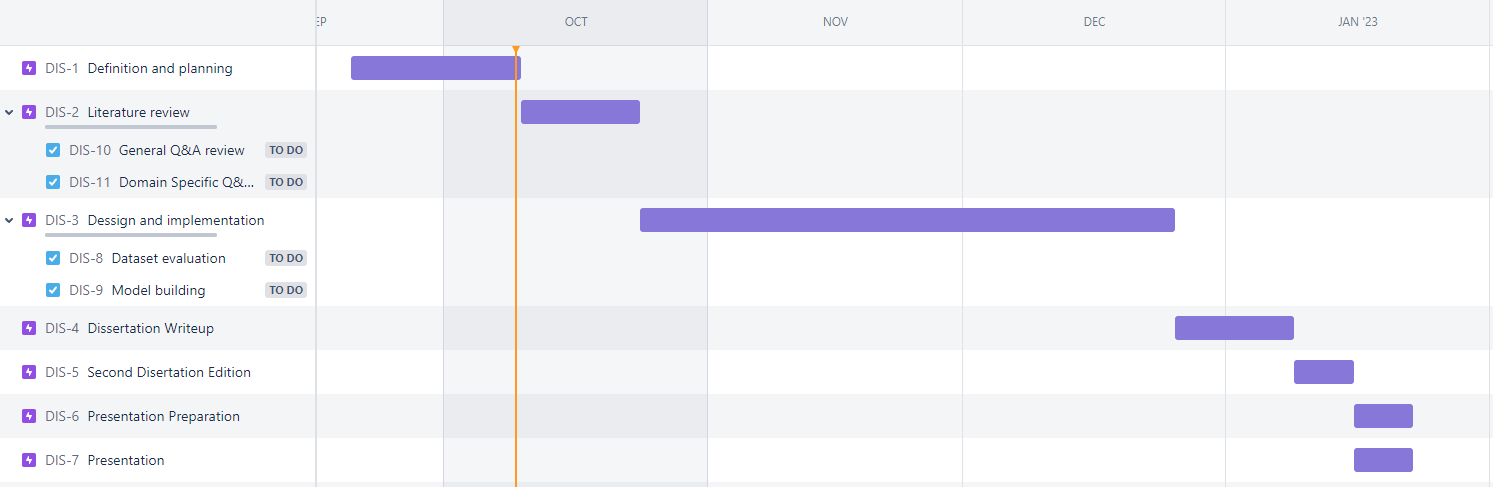
\includegraphics[width=16cm]{plan.png}
	\label{fig:gantt}
\end{figure}

\section{Global ethical commitment and Sustainable Development Objectives}
If the question answering accuracy is high enough, the project should reduce the turn-around time for mothers' queries, leading to better advice access for end users.
\subsection{Sustainability}
The main carbon footprint impact of the project will likely be in compute, given the size of the dataset, the likelihood is that the impact on the environment will be minor, given that the bulk of the work will be performed on a single, consumer grade hardware, workstation.
\subsection{Diversity and Inclusivity}
Active care will be taken to ensure that any biases present in the training data do not carry to the machine learning model. A more specific strategy will be devised after evaluating the training dataset.
\subsection{Ethical behaviour and social responsibility}
The data used will be anonymized and kept secure, limiting both the likelihood of data leaks, as well as mitigating the potential impact on the platform users. 

\chapter{Literature Review}


\label{chapter:literature_review}


\section{Introduction}
There are several methods to build question answering systems, this literature review focuses on document processing and answer processing, detailing the most common and latest techniques used when building the systems.

\section{Term similarity based QA}
Traditional search engines use terms in the search query to match the similarity of the question to the available documents. One of the first systems to implement term based search was Smart (System for the Mechanical Analysis and Retrieval of Text) \cite{10.5555/1102022}, developed in 1971, it used TF-IDF to rank the relevant documents for a query. Similar implementations of Smart have lead to successful open-source and commercial implementations like Lucene \cite{bialecki2012apache} or Elasticsearch \cite{elasticsearch2018elasticsearch}, which are widely used as single-website search engines \cite{andrews2005magic}. 

Term based searches can be further refined to extract passages within the documents, these can be defined to be individual sentences, series of sentences, or other pre-defined or dynamic lengths of text. There are several techniques to extract and rank the passages \cite{tellex2003quantitative}, which include: 
\begin{itemize}
	\item \textbf{MITRE}: Each individual sentence becomes a passage, and word overlap is used to rank them \cite{light2001analyses}.
	\item \textbf{MultiText}: The passage is determined by a variable sized window that starts and ends with a query term, creating passages of arbitrary length. The passages are ranked by inverse document frequency while penalizing longer passages \cite{clarke2000question}.
	\item \textbf{Alicante}: The passage length is parametrized at runtime, by specifying the number of sentences to be included in each overlapping window passage. Each window is then scored using cosine similarity between each sentence and the query's TF-IDF vector, as well as the similarity amongst the sentences within the passage \cite{vicedo2002university}.
\end{itemize}

\section{Natural Language Processing}
Layering Natural Language Processing techniques over traditional information retrieval methods adds nuance to the extraction. Multiple techniques can be used to improve results, encoding both the query and the potential passages:

\begin{itemize}
	\item \textbf{TF-IDF}: A non-contextual purely statistical methods use the relative frequency of a term when compared to the frequency of the same term over the whole corpus \cite{5392697}. While efficient and widely used, it does not use any external corpora to improve results. Cosine similarity is generally used between the encoded question vectors and the encoded passages.
	\item \textbf{Word2Vec}: The encoder is built by training a shallow neural network to learn word associations based on their context \cite{mikolov2013efficient}. The vectors can be trained on a large external corpus, on the target documents containing the potential answer, or on a combination of both. The vectors of all the words in a given passage can be aggregated with Doc2Vec \cite{le2014distributed}, by averaging or concatenating them, and appending a paragraph ID.
	\item \textbf{BERT}: This open source framework, Bidirectional Encoder Representations from Transformers \cite{devlin2018bert}, uses a combination of two techniques to encode passages: Masked Language Modelling, where the model is trained to predict the missing word on a given sentence; and Next Sentence Prediction, where the model is trained to predict the sentence after the current one. BERT can be further fine-tuned to the specific corpora to improve question answering quality on restricted domains.
\end{itemize}

These techniques can be used individually or in conjunction to build a question answering pipeline.

\section{Knowledge Base QA}
Knowledge Base Question Answering works with the potential answer in structured data instead of unstructured documents. These systems rely on translating unstructured questions to database queries. Questions have to be first categorized by their goal \cite{YANG20159086}, e.g. is it a "who" question or a "what" question, named entities are then extracted from the question, and the combination of those is used to map a predicate to be extracted from the knowledge base.



% bibliografia
\addcontentsline{toc}{chapter}{References}
\bibliographystyle{plain}
\bibliography{referencias}

\end{document}